\section{Distributed Machine Learning}
%%%%%%%%%%%%%%%%%%%%%%%%%%%%%%%%%%%%%%%%%%%%%%%%%%%%%%%%%%%%%%%%%%%%%%%%%%%%%%%%%%%%%%%%%%%%%%%%%%%%%%%%%%%%%%%%%%%%%%%%%%%%%%%%%%%%%%%%%%%%%%%%%%%%%%%%%%%%%%
\subsection{The Need for Distribution}
As the field of machine learning (ML) continues to evolve, the demand for processing vast amounts of data and training
increasingly complex models has surged. Traditional machine-learning methodologies, which typically operate on single-machine setups,
face significant limitations in terms of computational power and memory capacity. This led, in the past, to the development and adoption of
centralized learning approaches, where data from various sources is aggregated into a central location for processing. While centralized
learning mitigates some of the constraints of single-machine learning, it still struggles with issues such as data transfer overhead,
security risks, and the inability to scale efficiently with ever-growing datasets.

To overcome these shortcomings, the paradigm has shifted towards Distributed Machine Learning (DML). DML allows for the distribution of data
and computational tasks across multiple machines or devices, leveraging their collective resources. This approach not only enhances
computational efficiency through parallelism, but also enables the processing of larger datasets that would be infeasible for centralized systems.
By distributing the workload, DML restricts data transfer bottlenecks, enhances fault tolerance, and provides greater scalability, making it an essential
advancement for modern machine learning applications.


\begin{figure}[!ht]
    \centering
    \begin{subfigure}[b]{0.49\textwidth}
        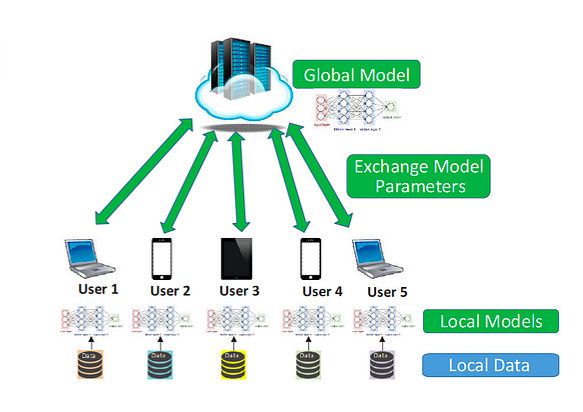
\includegraphics[height=.8\textwidth,keepaspectratio]{figures/dml/distributed_1.png}
        \caption{Distributed Learning}
        \label{fig:distributed}
    \end{subfigure}
    \hfill
    \begin{subfigure}[b]{0.49\textwidth}
        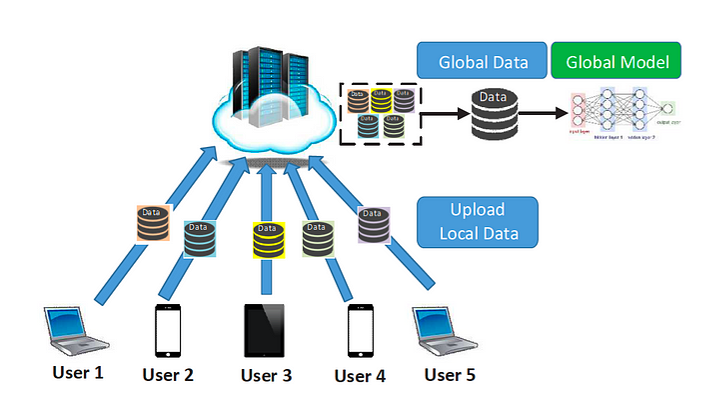
\includegraphics[height=.8\textwidth,keepaspectratio]{figures/dml/centralized.png}
        \caption{Centralized Learning}
        \label{fig:centralized}
    \end{subfigure}
    \caption{A comparison between distributed and centralized learning approaches}
    \label{fig:centralized_vs_distributed}
\end{figure}

Thus, the progression from traditional ML to centralized learning, and finally to DML, reflects the ongoing need to optimize and scale
machine learning processes to keep pace with the increasing data demands and computational complexities of contemporary applications.
%%%%%%%%%%%%%%%%%%%%%%%%%%%%%%%%%%%%%%%%%%%%%%%%%%%%%%%%%%%%%%%%%%%%%%%%%%%%%%%
%%%%%%%%%%%%%%%%%%%%%%%%%%%%%%%%%%%%%%%%%%%%%%%%%%%%%%%%%%%%%%%%%%%%%%%%%%%%%%%%%%%%%%%%%%%%%%%%%%%%%%%%%%%%%%%%%%%%%%%%%%%%%%%%%%%%%%%%%%%%%%%%%%%%%%%%%%%%%%
\subsection{Distributed Learning Systems Architecture}
\label{sec:dml_architecture}
The architecture of DML Systems can be defined by a triad of layers dependent on each other: \emph{The Distribution Method (Parallelism)},
\emph{the System's Communication Topology}, and \emph{the ML algorithm}. A broad overview of the above will be presented as follows:

%%%%%%%%%%%%%%%%%%%%%%%%%%%%%%%%%%%%%%%%%%%%%%%%%%%%%%%%%%%%%%%%%%%%%%%%%%%%%%%
\subsubsection{Parallelism in Distributed Learning Systems}\label{sec:parallelism}
Parallelism in DML Systems can be achieved with two methods; Data and Model Parallelism.
A thorough survey by Joost Verbraeken et al.\cite{joostverbraekenSurveyDistributedMachine} clarifies:
\begin{itemize}
    \item \emph{Data Parallelism:} In the data-parallel approach, the dataset is divided into segments corresponding to the number of worker nodes
          in the system. Each worker node then processes its respective data segment using the same algorithm. The model is either centralized or replicated
          across all worker nodes, ensuring a unified output. This method is applicable to any machine learning algorithm that assumes independent and
          identical distribution (i.i.d.) of data samples, which includes the majority of ML algorithms.

    \item \emph{Model Parallelism:} Model parallelism involves splitting the model itself across multiple machines and training different parts of the model
          on different machines. This approach is useful when the model is too large to fit in the memory of a single machine, or when certain parts of the model
          require more computation than others. Model parallelism is a bit more complex to implement and is less common than data parallelism, but is still used in
          some specialized applications, as it cannot automatically be applied to every machine learning algorithm because the model parameters generally cannot be split up.
\end{itemize}

\begin{figure}[!ht]
    \centering
    \begin{subfigure}[b]{0.45\textwidth}
        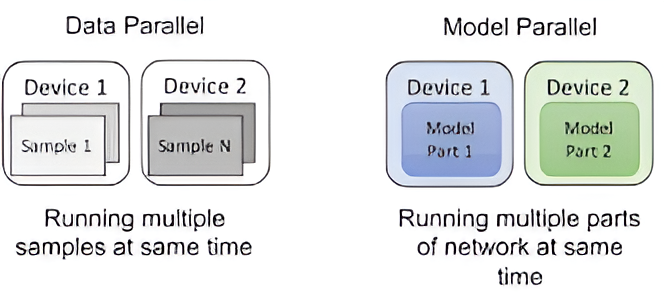
\includegraphics[width=\textwidth]{figures/dml/parallelism_1_1716025674884.png}
        \caption{Parallelism logic depiction}
        \label{fig:parallelism_method}
    \end{subfigure}
    \hfill
    \begin{subfigure}[b]{0.45\textwidth}
        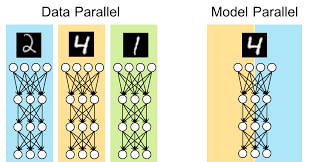
\includegraphics[width=\textwidth]{figures/dml/parallelism.png}
        \caption{An example of model and data parallelism}
        \label{fig:parallelism_example}
    \end{subfigure}
    \caption{Data and Model Parallelism Methods}
    \label{fig:parallelism}
\end{figure}

%%%%%%%%%%%%%%%%%%%%%%%%%%%%%%%%%%%%%%%%%%%%%%%%%%%%%%%%%%%%%%%%%%%%%%%%%%%%%%%
\subsubsection{Distributed Systems Communication Topologies}\label{sec:dml_topologies}
In DML, the communication architecture delineates the specific roles of training nodes. These roles include computation nodes, which compute gradients,
and parameter aggregation nodes, responsible for aggregating these gradients and updating the model parameters. Additionally, it defines the logical
topologies for node communication, such as star or ring configurations. Regardless of the model type and learning objective, the same communication
architecture facilitates parameter exchange and synchronization when using gradient-based optimization algorithms. A Recent article from Liu et al.
~\cite{liuTopologiesDistributedMachine2024} showcases the three primarily used connectivities in Distributed Systems.

\begin{figure}[!ht]
    \centering
    \begin{subfigure}[b]{0.45\textwidth}
        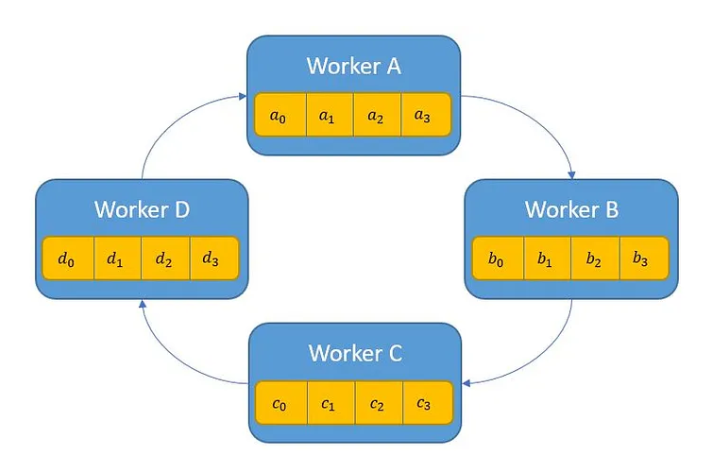
\includegraphics[width=\textwidth]{figures/dml/ring.png}
        \caption{Ring-All Reduce}
        \label{fig:ring}
    \end{subfigure}
    \hfill
    \begin{subfigure}[b]{0.45\textwidth}
        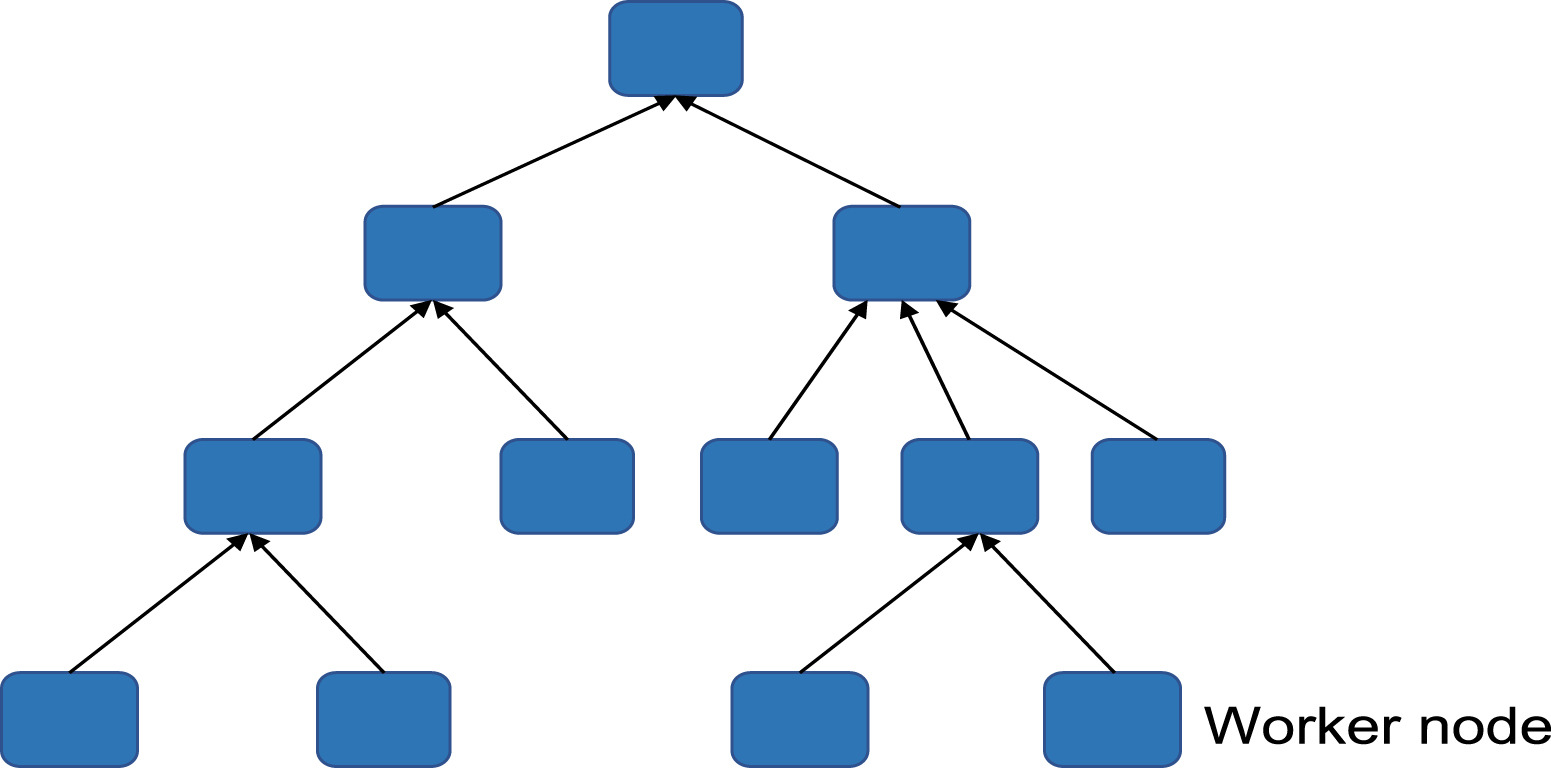
\includegraphics[width=\textwidth, height=0.6\textwidth]{figures/dml/tree.jpg}
        \caption{Hierarchical-Tree}
        \label{fig:tree}
    \end{subfigure}
    \begin{subfigure}[b]{0.6\textwidth}
        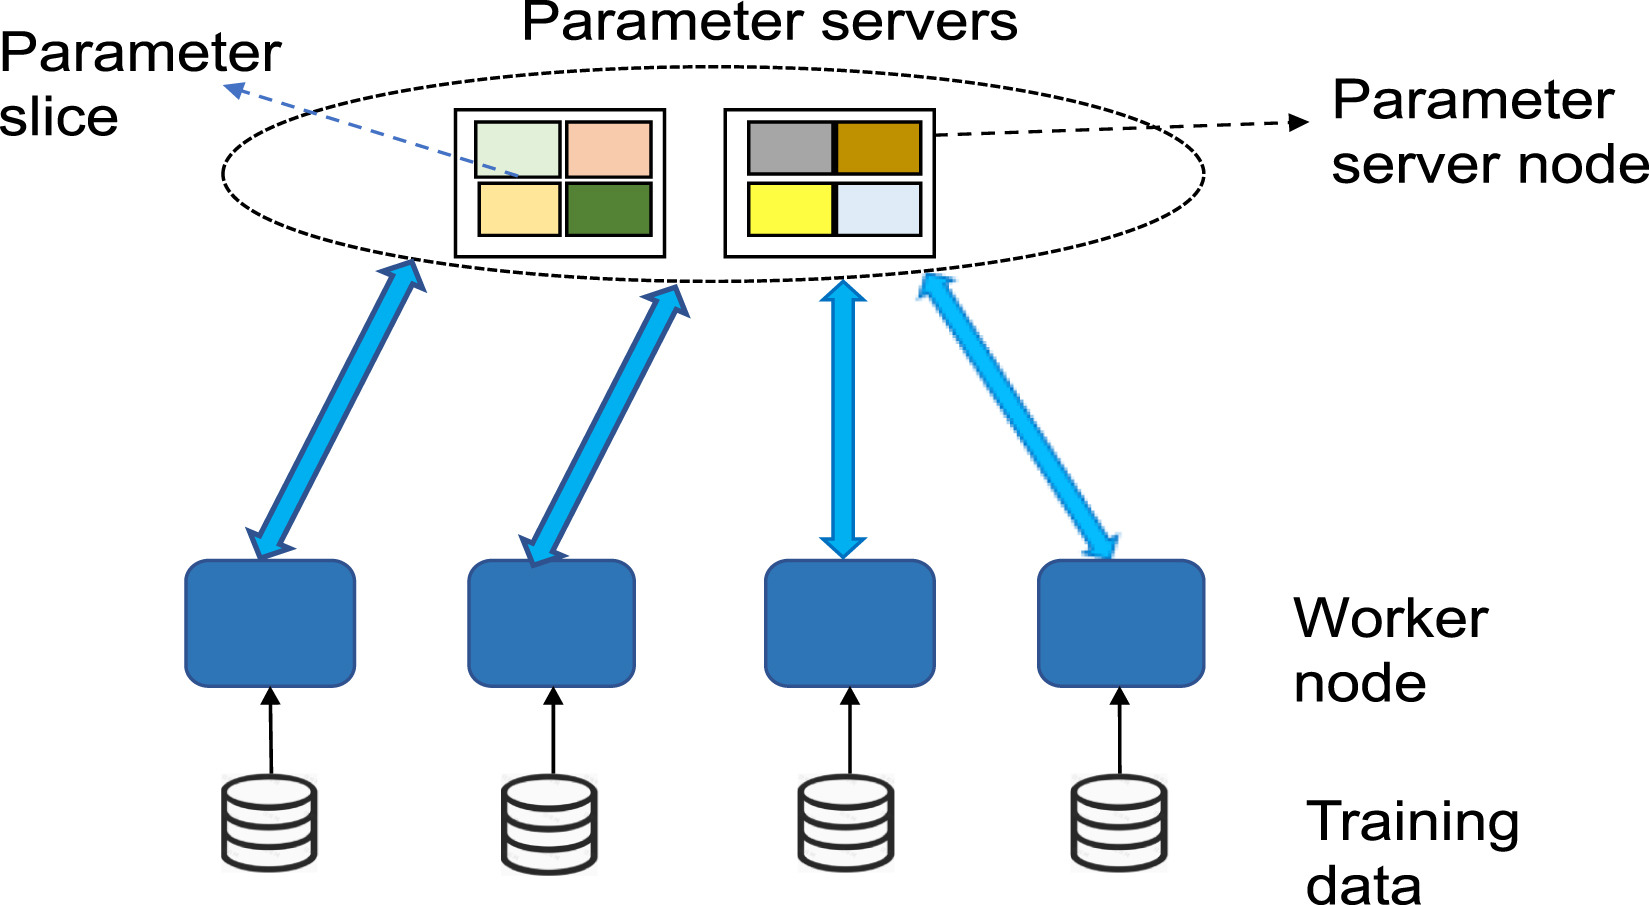
\includegraphics[width=\textwidth]{figures/dml/parameter_server_1.jpg}
        \caption{Decentralized-Parameter Server}
        \label{fig:parameter_server}
    \end{subfigure}
    \caption{Principle Distributed Systems Communication Topologies}
    \label{fig:topologies}
\end{figure}

\begin{itemize}
    \item \emph{Ring-All Reduce:} The Ring architecture arranges nodes in a ring topology, where each node communicates directly with its two neighbors.
          Gradients are shared in a circular manner, with each node sending and receiving data from its adjacent nodes. This architecture efficiently
          utilizes bandwidth by limiting communication to neighboring nodes and avoids the bottlenecks of a centralized coordinator. It is particularly effective
          in GPU clusters and is widely used in distributed deep learning frameworks. A notable example of this topology is the Ring-All Reduce
          implementation provided by Uber's Horovod framework\cite{sergeevHorovodFastEasy2018}.
    \item \emph{Hierarchical-Tree:} The Hierarchical-Tree architecture organizes nodes in a tree structure, where intermediate nodes aggregate gradients
          from their child nodes and pass the aggregated results up the tree to the root node. This reduces the communication overhead compared to a fully
          connected topology and scales efficiently with the number of nodes. The root node eventually computes the global model update and propagates it back
          down the tree. This architecture provides a balance between scalability and communication efficiency\cite{ReillyNetworkDistributed}.
    \item \emph{Decentralized-Parameter Server:} The Decentralized-Parameter Server architecture involves multiple parameter servers distributing the
          management of model parameters. Each worker node communicates with one or more parameter servers to read and update parameters during training. This
          decentralization reduces mitigates bottlenecks and improves fault tolerance compared to a single centralized server. The architecture requires synchronization
          between parameter servers to ensure model consistency across the network.

          This connectivity architecture resembles most the research's implementation,
          yet is restricted to a singular server to mitigate cross-server communication challenges\footnote{Parameter server implementation with a singular server
              resembles a star architecture-all worker nodes directly connected to server}.
          In this scenario, all worker nodes directly communicate with the central server, simplifying network management and reducing latency in communication
          by having a single aggregation point. However, this also introduces a potential bottleneck at the central server and may suffer from single points of failure.
\end{itemize}

%%%%%%%%%%%%%%%%%%%%%%%%%%%%%%%%%%%%%%%%%%%%%%%%%%%%%%%%%%%%%%%%%%%%%%%%%%%%%%%
\subsubsection{Distributed Learning Algorithms}
Last but not least, The DML algorithm selection determines how the learning is conducted after \textit{parallelism method} and \textit{communication topology} are
established. The objective in DML algorithms always remains to leverage parallelism and efficient communication to accelerate training and enable the handling of
large datasets and models that are infeasible for single-machine setups. Therefore, to achieve their goal, data and computation loads are distributed across several
nodes-either being various accelerating devices like GPUs or TPUs or completely different machines\cite{teerapittayanonDistributedDeepNeural2017}.
An outline of an algorithm to achieve the above is presented:

\begin{enumerate}
    \item \emph{Data Preparation:} Partitioning the dataset into subsets that can be distributed across multiple worker nodes,
          ensuring that data distribution maintains the independent and identical distribution (i.i.d.) property when required.
    \item \emph{Model Initialization:} All local models are initialized either locally by each node or centrally by a server and distributed.
          Depending on the needs, the parameters initialization can be random or with a specific model state.
    \item \emph{Local Training:} Each worker node processes its assigned data subset to compute local gradients.
          Parallelism techniques (data parallelism or model parallelism, see \cref{sec:parallelism}) are applied to enhance computational efficiency.
    \item \emph{Gradient Aggregation \& Synchronization:}Gradients computed by each worker are sent either to a server or a peer for aggregation, depending on the topology,
          to update the global model (see \cref{sec:dml_topologies}). Synchronization can be synchronous or asynchronous, affecting the overall training dynamics.
    \item \emph{Model Update:} The updated global model is transmitted back to the worker nodes to reinstate the global
          parameter values to the local model.
    \item \emph{Iteration:} Steps 3 to 5 are repeated until the stopping condition is met.
\end{enumerate}

At this point, we should delve a little deeper into the \emph{Gradient Aggregation \& Synchronization} part outlined previously, in order to sufficiently cover the
principal matter of Synchronization in DML Systems. To be specific, Synchronization can be achieved either in Synchronous or Asynchronous manner in DML systems.
Each of these approaches inevitably comes with some merits and some challenges. In an effort to highlight those, the fundamental optimization algorithms for
gradient calculation, both in Synchronous and Asynchronous Synchronization-namely Synchronous SGD (SSGD) and Asynchronous SGD (ASGD), will be briefly demonstrated.

\paragraph{Synchronous SGD (SSGD)} In SSGD all worker nodes must complete their gradient computations and communicate these gradients before the global model parameters are updated.
This ensures consistency across model updates, as all nodes work with the same model parameters in each iteration. However, this approach can lead to inefficiencies due
to idle times when faster nodes wait for slower ones, also known as the straggler effect. This can impact scalability, especially in large distributed systems where node
performance can vary significantly. On final analysis, the rule to update the parameters, executed by the server at each iteration, can be summarized
~\cite{chenRevisitingDistributedSynchronous2017}:

\begin{equation}
    \label{eq:ssgd}
    w_{t+1} = w_t - \eta \cdot \frac{1}{K} \sum_{i=1}^{K} \nabla f_{\gamma_{t,i}}(w_t)
\end{equation}

Where in the rule above, \emph{$\eta$} denotes the learning rate, \emph{$K$} the number of workers, and \emph{$\gamma_{t,i}$} an index chosen uniformly
at random by the $i$-th worker from ${1,\dots,n}$, representing a selected data point\footnote{It is common in literature to present the SGD approach
    of the algorithm interchangeably with the Mini-Batch approach. This convention is also followed for this research's implementation, so clarification
    was necessary to avoid confusion.}. Thus,  \emph{$\nabla f_{\gamma_{t,i}}(w_t)$} is the stochastic
gradient estimate from the $i$-th worker for the \emph{$\gamma_{t,i}$} data point (or batch).

\paragraph{Asynchronous SGD (ASGD)}
ASGD, conversely, allows worker nodes to proceed with their computations and update model parameters independently of other nodes. This reduces
idle times and can lead to better utilization of computational resources, thereby enhancing scalability. However, the lack of synchronization can result in inconsistencies,
as updates may be based on stale gradients, potentially slowing down the convergence of the model or leading to convergence issues. In Summary, the update rule utilized
in ASSD is\cite{AsynchronousDecentralizedParallel}:

\begin{equation}
    \label{eq:asgd}
    w_{t+1} = w_t - \eta \nabla f_{\gamma_{t,i}}(w_{t - \tau_{i}})
\end{equation}

Where in the rule above, \emph{$\eta$} denotes the learning rate, \(\gamma_{t,i}\) is an index chosen uniformly at random by the \(i\)-th worker
from \(\{1,\dots,n\}\), representing a selected data point, \(\nabla f_{\gamma_{t,i}}(w_{t - \tau_{i}})\) is the stochastic gradient estimate from the
\(i\)-th worker for the \(\gamma_{t,i}\)-th data point, computed at a delayed iteration \( t - \tau_{i} \) due to asynchronous updates.

The choice between Synchronous and Asynchronous SGD is crucial in designing effective DML systems. Synchronous SGD is typically preferred when
consistency and simplicity are paramount, and the computational environment is relatively homogeneous, minimizing the straggler effect.
On the other hand, Asynchronous SGD is advantageous in heterogeneous environments where reducing idle time and improving resource utilization
is critical. The same applies to all the modified and improved variations stemming from these fundamental algorithms that comprise the
cornerstone of DML algorithm implementations.

Conluding, as stated at the beginning of this subsection \cref{sec:dml_architecture} the architecture of a DML system can be decomposed into
the three layers of emph{The Distribution Method (Parallelism)}, \emph{the System's Communication Topology} and \emph{the ML algorithm}. Therefore,
researchers and practitioners of the field need always be aware of the characteristics, both merits and challenges, various designing options
entail, in order to orchestrate efficient and useful DML Systems that can successfully satisfy the problem requirements.

%%%%%%%%%%%%%%%%%%%%%%%%%%%%%%%%%%%%%%%%%%%%%%%%%%%%%%%%%%%%%%%%%%%%%%%%%%%%%%%
%%%%%%%%%%%%%%%%%%%%%%%%%%%%%%%%%%%%%%%%%%%%%%%%%%%%%%%%%%%%%%%%%%%%%%%%%%%%%%%%%%%%%%%%%%%%%%%%%%%%%%%%%%%%%%%%%%%%%%%%%%%%%%%%%%%%%%%%%%%%%%%%%%%%%%%%%%%%%%
\subsection{Challenges in Distributed Machine Learning}
\label{sec:dml_challenges}
Distributed Machine Learning (DML) offers significant advantages in processing large datasets and complex models by leveraging parallelism and
distributed resources. However, it also introduces several challenges, some of which are depicted in \cref{tab:dml_challenges}, that can impact efficiency,
scalability, consistency, and security. These challenges are critical to understand as they set the stage for the transition to Federated
Learning (FL), which addresses several of these issues.

\begin{table}[h!]
    \centering
    \begin{tabular}{>{\raggedright}p{4cm} >{\raggedright}p{7cm} >{\raggedright\arraybackslash}p{3cm}}
        \toprule
        \rowcolor{lightgray}
        \textbf{Challenge}     & \textbf{Description}                                                                                                                                                   & \textbf{Addressed by FL} \\
        \midrule
        Communication Overhead & Frequent communication for gradient updates and synchronization can lead to significant overhead, particularly in environments with limited bandwidth or high latency. & Yes                      \\
        \midrule
        Privacy and Security   & Distributed systems are vulnerable to privacy breaches and security attacks, as data is transferred across nodes and potentially exposed to unauthorized access.       & Yes                      \\
        \midrule
        Data Heterogeneity     & Data distributed across nodes may not be identically and independently distributed (non-IID), leading to biases and inconsistencies in model training.                 & Yes                      \\
        \midrule
        Scalability            & Managing communication and synchronization efficiently becomes challenging as the number of nodes increases, potentially incurring high costs.                         & Partially                \\
        \midrule
        Fault Tolerance        & Ensuring reliability and fault tolerance in a distributed setting is complex, requiring robust mechanisms to handle node failures and network disruptions.             & No                       \\
        \midrule
        Straggler Effect       & In synchronous training, faster nodes must wait for slower ones, leading to idle times and inefficient resource utilization.                                           & No                       \\
        \bottomrule
    \end{tabular}
    \caption{Challenges of Distributed Machine Learning}
    \label{tab:dml_challenges}
\end{table}


\paragraph{Transition to Federated Learning}
Federated Learning (FL) builds on the principles of DML but addresses many of its inherent challenges, particularly those related
to data privacy, communication overhead, and data heterogeneity. To demonstrate, By preserving the training dataset locally Federated Learning
never utilizes the network for private data transmission, negating that way any ill-advised privacy infringements. Moreover, By enabling
local training on edge devices and aggregating only the necessary updates at the end of a learning round, FL restricts network utilization
and additionally enhances privacy. It should be noted also, that Federated Learning systems do not function under the assumption of i.i.d.
data which frequently cannot be stated for other DML system setups. Finally, scalability is partially enhanced due to the overall resetriction
of communication overheads, as only model update transmission are executed and no data transfers leading to more system resources being available,
then again, this performance improvement cannot be objectively measured and in some cases is negligible.

This transition from DML to FL represents an evolution towards more efficient, scalable,
and secure machine learning practices, leveraging distributed resources while mitigating the traditional challenges of DML systems.
In summary, the challenges of DML portrayed at \cref{tab:dml_challenges} highlight the need for more advanced approaches like
Federated Learning. FL addresses these issues by enabling decentralized data processing and focusing on privacy-preserving methods,
making it a crucial advancement for modern machine learning applications, as will be further illustrated in the next section.